%********** Chapter 4 **********
\chapter{Kinect Device}

\section{Introduction}

Kinect is a motion sensing input device by Microsoft for the Xbox 360 video game console and Windows PCs. Based around a webcam-style add-on peripheral for the Xbox 360 console, it enables users to control and interact with the Xbox 360 without the need to touch a game controller, through a natural user interface using gestures and spoken commands.
Kinect was launched in North America on November 4, 2010, in Europe on November 10, 2010, in Australia, New Zealand and Singapore on November 18, 2010, and in Japan on November 20, 2010. 
Microsoft released Kinect software development kit for Windows 7 on June 16, 2011. 
This SDK allows developers to write Kinecting apps in C++/CLI, C\# or Visual Basic .NET

\begin{figure}[H]
\centering
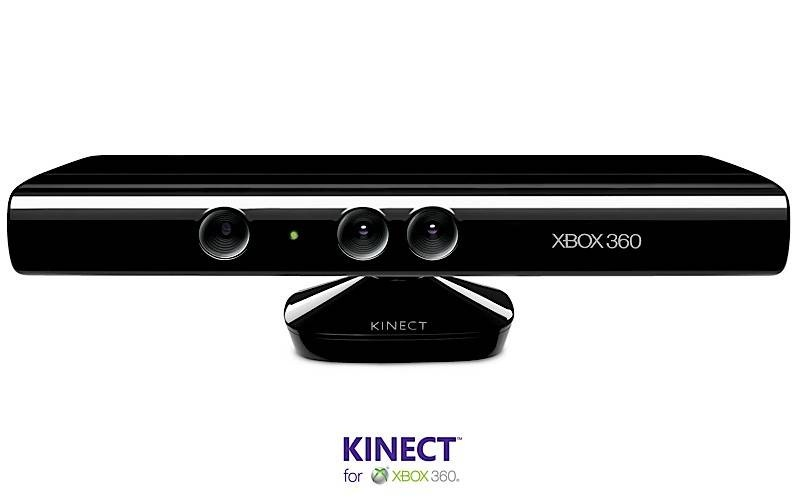
\includegraphics[scale=0.4,keepaspectratio=true]{Kinect/kinect.jpg}
\caption{Kinect for Xbox 360}
\label{fig:kinect}
\end{figure}

\section{Technology}

Kinect builds on software technology developed internally by Rare, a subsidiary of Microsoft Game Studios owned by Microsoft, and on range camera technology, which developed a system that can interpret specific gestures, making completely hands-free control of electronic devices possible by using an infrared projector and camera and a special microchip to track the movement of objects and individuals in three dimension. 
This 3D scanner system called Light Coding employs a variant of image-based 3D reconstruction.
The depth sensor consists of an infrared laser projector combined with a monochrome CMOS sensor, which captures video data in 3D under any ambient light conditions. 
The sensing range of the depth sensor is adjustable, and the Kinect software is capable of automatically calibrating the sensor based on gameplay and the player's physical environment, accommodating for the presence of furniture or other obstacles.

\begin{figure}[H]
\centering
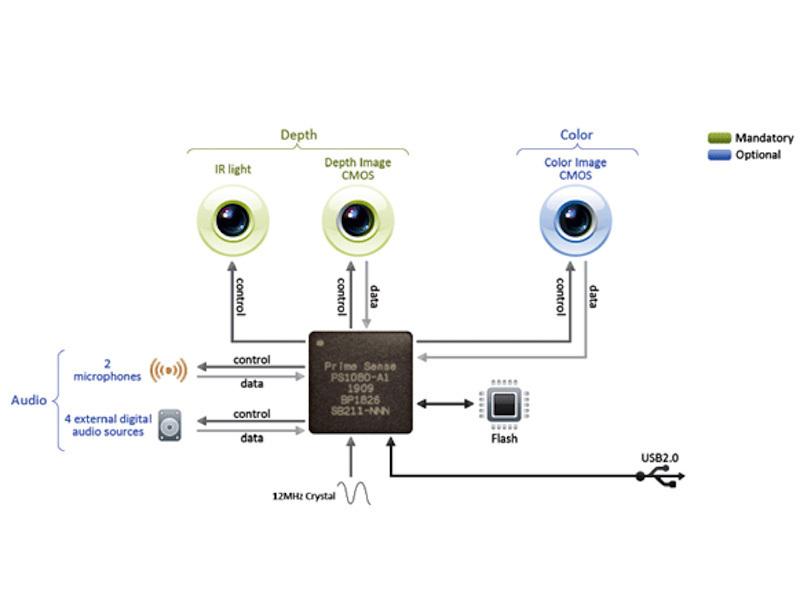
\includegraphics[scale=0.6,keepaspectratio=true]{Kinect/kinect_technology.jpg}
\caption{Underlying technology of Kinect }
\label{fig:kinect_technology}
\end{figure}

\section{Depth Image}

Kinect captures a sequence of two types of synchronized frames, an RGB Image and a depth Image, the synchronization between the two images ensures that each RGB image has a correspondent depth image.
Using information obtained from each two synchronized frames, we can obtain for each pixel:
\begin{itemize}
\item  RGB color information
\item $x$ ,$y$ and $z$ co-ordinates 
\end{itemize}


RGB image is a simple  640$\times$480 pixels image
Depth image is a 640$\times$480 pixels grayscale image where:
\begin{itemize}
\item Bright colors represent close objects
\item Dark colors represent far objects
\item Black segments represent objects out of range "too close or too far"
\end{itemize}

\begin{figure}[H]
\centering
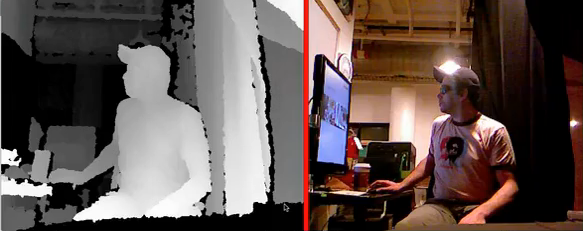
\includegraphics[scale=1,keepaspectratio=true]{Kinect/kinect_depth.png}
\caption{A figure showing depth color on the left with its correspondent RGB image, the brighter the pixel the closer it is, while out of range pixels are represented in black}
\label{fig:kinect_depth}
\end{figure}

\section{Device Specifications}

\begin{table}[H]
\centering
\begin{tabular}{|l|l|}
  \hline
  Sensor & Colour and depth-sensing lenses \\
   & Voice microphone array \\
   & Tilt motor for sensor adjustment \\
   & Fully compatible with existing Xbox 360 consoles\\
  \hline
  Field of View & Horizontal field of view: 57 degrees\\
	    & Vertical field of view: 43 degrees\\
       & Physical tilt range: � 27 degrees\\
       & Depth sensor range: 1.2m - 3.5m\\
  \hline
  Skeletal Tracking System & Tracks up to 6 people, including 2 active players \\
  & Tracks 20 joints per active player \\
  & Ability to map active players to LIVE Avatars \\

  \hline
Audio System & LIVE party chat and in-game voice chat \\
             & Echo cancellation system enhances voice input \\
             & Speech recognition in multiple \\
  \hline
Camera resolution & 640 * 480\\
                  & 320 * 240\\
  \hline
Frame rate & 30 frames per second\\
  \hline

\end{tabular}
\caption{Kinect Specifications}
\label{tab:kinect_specs}
\end{table}

\pagebreak
\section{Why Kinect?}

\subsection{Capturing the depth}

As mentioned earlier Kinstruct is all about capturing a sequence of frames for a scene and building a 3D model from the processing of those frames, if we have information about $x$ ,$y$ and $z$ co-ordinates for each pixel in a frame in the real world, then it would be much more easier to align frames and distinguish between overlapping objects.

\subsection{Price and Availability}

The preference of the Kinect sensor comes from its affordable price according to other distance detectors that uses different technologies, also the Kinect functions as both a camera and a depth sensor, so there's no need to afford two different hardware devices.


\begin{table}[H]
\centering
\begin{tabular}{{|l|l|l|}}

  \hline
  Device & Kinect & Laser sensor \\
  \hline
  Cost & \$150 & \$45000 - \$60000  \\
  \hline 
  Availability & Electronics store & Need to order \\
  \hline
  Programmable interface & High level & Low level \\
  \hline
 
\end{tabular}
\caption{Kinect Specifications}
\label{tab:kinect_specs}
\end{table}


\pagebreak
\section{Precision of the Kinect sensor}

Because the Kinect is essentially a stereo camera, the expected error on its depth measurements is proportional to the distance squared. 

The experimental data shown in the graph below confirms the expected error model. 
The graph was obtained by pointing the Kinect at a planar surface, fitting a plane (using RANSAC) through the measured point cloud, and checking the distance of the points in the point cloud to that plane. This means the plane represents the average distance measurement, and the graph shows how far off the Kinect measurements are from that average distance.

\begin{figure}[H]
\centering
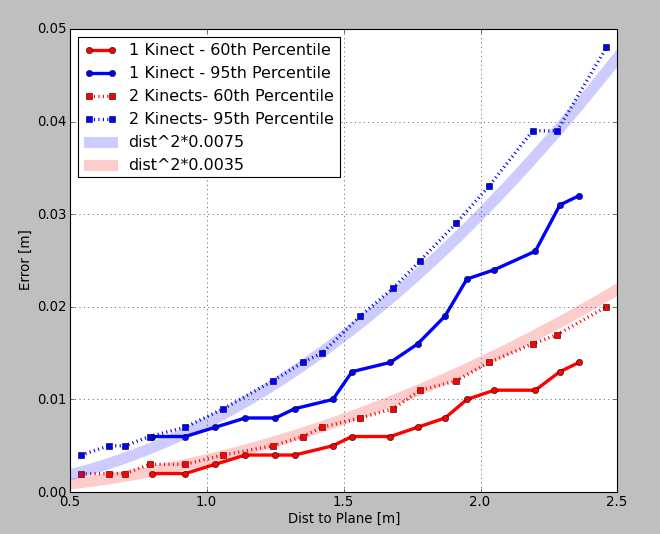
\includegraphics[scale=0.6,keepaspectratio=true]{Kinect/precision.png}
\caption{Precision of the Kinect measuring depth}
\label{fig:precision}
\end{figure}

\section{Kinect SDKs}

\subsection{Kinect SDK for Windows}
The Kinect for Windows SDK enables developers to create applications using C++, C\# or Visual Basic, which support gesture and voice recognition using the Kinect for Windows sensor and a PC or embedded device.

It includes drivers for using Kinect sensor on a computer running Windows 7, Windows 8 Consumer Preview, and Windows Embedded Standard 7. In addition, the download includes application programming interfaces (APIs) and device interfaces.

\subsection{Open Kinect}

OpenKinect is an open community of people interested in making use of the Xbox Kinect hardware with our PCs and other devices. 
Working on free, open source libraries that will enable the Kinect to be used with Windows, Linux, and Mac.

\subsection{Open NI}

OpenNI or Open Natural Interaction is an industry-led, non-profit organization focused on certifying and improving interoperability of natural user interface and organic user interface for natural interaction devices, applications that use those devices and middleware that facilitates access and use of such devices.

The organisation has been created on November 2010, with the website going public on December 8th. One of the main members is PrimeSense, the company behind the technology used in the Kinect, a motion sensing input device by Microsoft for the Xbox 360 video game console.

In December 2010, PrimeSense, whose depth sensing reference design Kinect is based on, released their own open source drivers along with motion tracking middleware called NITE.PrimeSense later announced that it had teamed up with Asus to develop a PC-compatible device similar to Kinect, which will be called Wavi Xtion and is scheduled for release in the second quarter of 2012
Natural Interaction Devices or Natural Interfaces are devices that capture body movements and sounds to allow for a more natural interaction of users with computers in the context of a Natural user interface. The Kinect and Wavi X-tion are examples of such devices.
